% chapter9_critical_evaluation.tex

\section{Chapter Overview}
This chapter presents a critical evaluation of the RootLens system through multiple perspectives: a self-evaluation by the developer, feedback from domain and technical experts, and an assessment of the degree to which functional and non-functional requirements were satisfied. The evaluation methodology is described, evaluators are identified, and the results are analysed to provide an honest appraisal of the system's strengths and limitations.

\section{Evaluation Methodology and Approach}
The critical evaluation employed three complementary methods to assess RootLens from different perspectives:

\begin{enumerate}
    \item \textbf{Self-Evaluation:} A reflective assessment by the developer based on the research questions, design goals, and implementation outcomes documented in earlier chapters.
    \item \textbf{Expert Evaluation:} Structured feedback from domain experts (DevOps/SRE practitioners) and technical experts (software engineers with Kubernetes experience) collected via a Google Form questionnaire distributed alongside a system demonstration video.
    \item \textbf{Requirements Traceability:} A systematic review of functional and non-functional requirements against their implementation status, linking each requirement to the evidence of its fulfilment.
\end{enumerate}

This multi-perspective approach ensures the evaluation captures both the developer's informed perspective and independent external assessments.

\section{Evaluation Criteria}
The evaluation criteria were derived from the research questions and non-functional requirements defined in Chapter~1 and Chapter~4 respectively:

\begin{table}[H]
\centering
\begin{tabularx}{\textwidth}{|l|X|X|}
\hline
\textbf{Criterion} & \textbf{Description} & \textbf{Target} \\ \hline
Root Cause Accuracy & Correct identification of the primary delay category (NFR02) & $\geq$ 95\% \\ \hline
Sub-Cause Accuracy & Correct identification of the specific sub-cause (NFR03) & $\geq$ 80\% \\ \hline
Diagnostic Latency & End-to-end time for hybrid diagnosis (NFR01) & $<$ 300ms \\ \hline
Confidence Calibration & Monotonic relationship between confidence and accuracy & High-confidence $>$ low-confidence accuracy \\ \hline
System Usability & Clarity and actionability of diagnostic outputs & Positive expert feedback \\ \hline
Industry Relevance & Practical applicability to real DevOps workflows & Positive expert feedback \\ \hline
\end{tabularx}
\caption{Critical Evaluation Criteria}
\label{tab:eval_criteria}
\end{table}

\section{Self-Evaluation}
This section provides an honest assessment of the system from the developer's perspective, informed by the full development and testing process.

\subsection{Strengths}
The hybrid rule-ML architecture proved to be a sound design decision. The rule-based engine provides deterministic, explainable primary classification at 96.7\% accuracy, while the ML explainers add sub-cause granularity (86.7\%) that would be impractical to achieve with rules alone. The graceful degradation mechanism ensures the system remains operational even when the ML service is unavailable, which is essential for a production diagnostic tool.

The 60/40 confidence combination model produces well-calibrated outputs: high-confidence predictions ($>$0.80) achieved 100\% accuracy, while low-confidence predictions ($<$0.70) achieved 75\%. This calibration property is arguably more operationally valuable than raw accuracy, as it enables risk-informed diagnostic decisions.

The use of real fault-injection data for model training, rather than purely synthetic data, strengthens the validity of the evaluation results. Each training sample corresponds to a verified Kubernetes failure scenario with ground-truth labels.

\subsection{Weaknesses}
The training dataset of 34-42 samples per category is small by ML standards. While the controlled experimental setup produced clean, well-separated data, this limits confidence in generalisation to production environments where failures are less cleanly separated and may co-occur.

The single misclassification in root cause accuracy occurred when scheduling contention and metric propagation lag co-occurred. The priority-ordered decision tree cannot express multi-cause scenarios, revealing a structural limitation of the taxonomy. A multi-label classification approach would address this but was beyond the project scope.

The fixed timing thresholds ($D_{cold} > 30s$, $D_{sched} > 10s$, $D_{lag} > 45s$) were calibrated on a single Minikube cluster. Production environments with different hardware, network characteristics, or cluster sizes would require threshold recalibration.

\subsection{Research Questions Assessment}
\textbf{RQ1:} Three timing signals classify the dominant root cause with 96.7\% accuracy. The thresholds were derived from Kubernetes and KEDA documentation, informed by experimental observation.

\textbf{RQ2:} Category-specific feature sets of 15, 11, and 10 features characterise sub-cause distinctions with 86.7\% overall accuracy. Feature importance analysis consistently identified the top discriminative features, validating the feature engineering decisions.

\textbf{RQ3:} The 60/40 rule-ML weighting produces well-calibrated confidence with monotonic calibration confirmed. Alternative weightings (50/50 and 70/30) were tested and found to be inferior.

\textbf{RQ4:} The hybrid approach matches rule-only root cause accuracy while adding sub-cause capability, and exceeds ML-only root cause accuracy (90.0\%). The 177ms latency trade-off is acceptable for diagnostic dashboards.

\section{Selection of the Evaluators}
Evaluators were selected based on their professional experience with Kubernetes and cloud-native systems. The evaluation was conducted using a structured Google Form distributed alongside a system demonstration video. Ten responses were received from practitioners across industry and academia. Table~\ref{tab:evaluators} profiles each evaluator.

\vspace{1em}

The Google Form questionnaire and the accompanying shared materials, including the demonstration video, are provided in Appendix~\ref{appendix:evaluation_materials} for reference.

\begin{xltabular}{\textwidth}{|p{1.2cm}|p{4cm}|X|p{3cm}|}

\hline
\textbf{ID} & \textbf{Position} & \textbf{Affiliation} & \textbf{Criteria} \\ \hline
\endfirsthead

\hline
\textbf{ID} & \textbf{Position} & \textbf{Affiliation} & \textbf{Criteria} \\ \hline
\endhead

EV1 & Senior DevOps Engineer & Industry (Altrium) & Technical Expert \\ \hline
EV2 & Senior DevOps Engineer & Industry (Creative Software) & Domain Expert \\ \hline
EV3 & Senior DevOps Engineer & Industry (Sysco Labs) & Domain Expert \\ \hline
EV4 & Senior DevOps Engineer & Industry (Sysco Labs) & Domain Expert \\ \hline
EV5 & Tech Lead & Industry (Sysco Labs) & Technical Expert \\ \hline
EV6 & DevOps Engineer & Industry (Altrium) & Domain Expert \\ \hline
EV7 & Senior SRE & Industry (Sysco Labs) & Domain Expert \\ \hline
EV8 & DevOps Engineer & Industry (Sysco Labs) & Domain Expert \\ \hline
EV9 & Associate AI/ML Engineer & Industry (Altrium) & Technical Expert \\ \hline
EV10 & Senior DevOps Engineer & Industry (Sysco Labs) & Technical Expert \\ \hline

\caption{Evaluator Profiles}
\label{tab:evaluators}
\end{xltabular}

\section{Evaluation Results}

This section presents the findings from the expert evaluation of \textbf{RootLens}, focusing on both quantitative ratings and qualitative feedback collected through the questionnaire.

Figure~\ref{fig:overall_impression} summarises the overall impression of RootLens as a diagnostic tool. The results indicate a highly positive response from participants, with all evaluators rating the system between 4 and 5 on a 5-point Likert scale. Specifically, 60\% of respondents rated the system as 5 (excellent), while the remaining 40\% rated it as 4 (good). Notably, no neutral or negative responses were recorded.

This strong consensus suggests that RootLens is perceived as an effective and valuable solution for diagnosing scaling delays in Kubernetes-based systems. The absence of low ratings further reinforces the system’s reliability and practical relevance to real-world DevOps and SRE workflows.

To provide a comprehensive evaluation, the findings are analysed in two dimensions: \textbf{quantitative analysis}, which examines the Likert-scale responses across key evaluation criteria, and \textbf{qualitative analysis}, which explores detailed feedback from participants regarding system clarity, limitations, integration potential, and suggested improvements.

\begin{figure}[H]
\centering
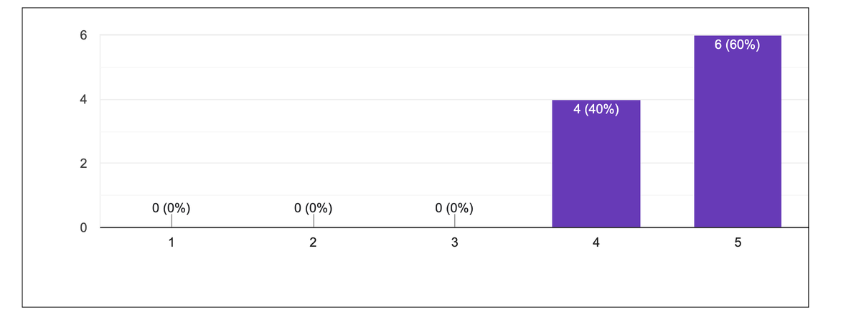
\includegraphics[width=0.8\textwidth]{thesis/assets/overall_impression.png}
\caption{Overall Impression of RootLens as a Diagnostic Tool}
\label{fig:overall_impression}
\end{figure}

\subsection{Quantitative Analysis}
Evaluators rated four dimensions on a 5-point Likert scale (1=Strongly Disagree, 5=Strongly Agree). Table~\ref{tab:likert_results} summarises the responses. Refer to the following table.

\begin{xltabular}{\textwidth}{|X|X|}
\hline
\textbf{Feedback} & \textbf{Justification} \\ \hline
\endfirsthead

\hline
\textbf{Feedback} & \textbf{Justification} \\ \hline
\endhead

\hline
\caption{Questionnaire for Industry Professionals}
\label{tab:questionnaire_industry}
\endlastfoot

\centering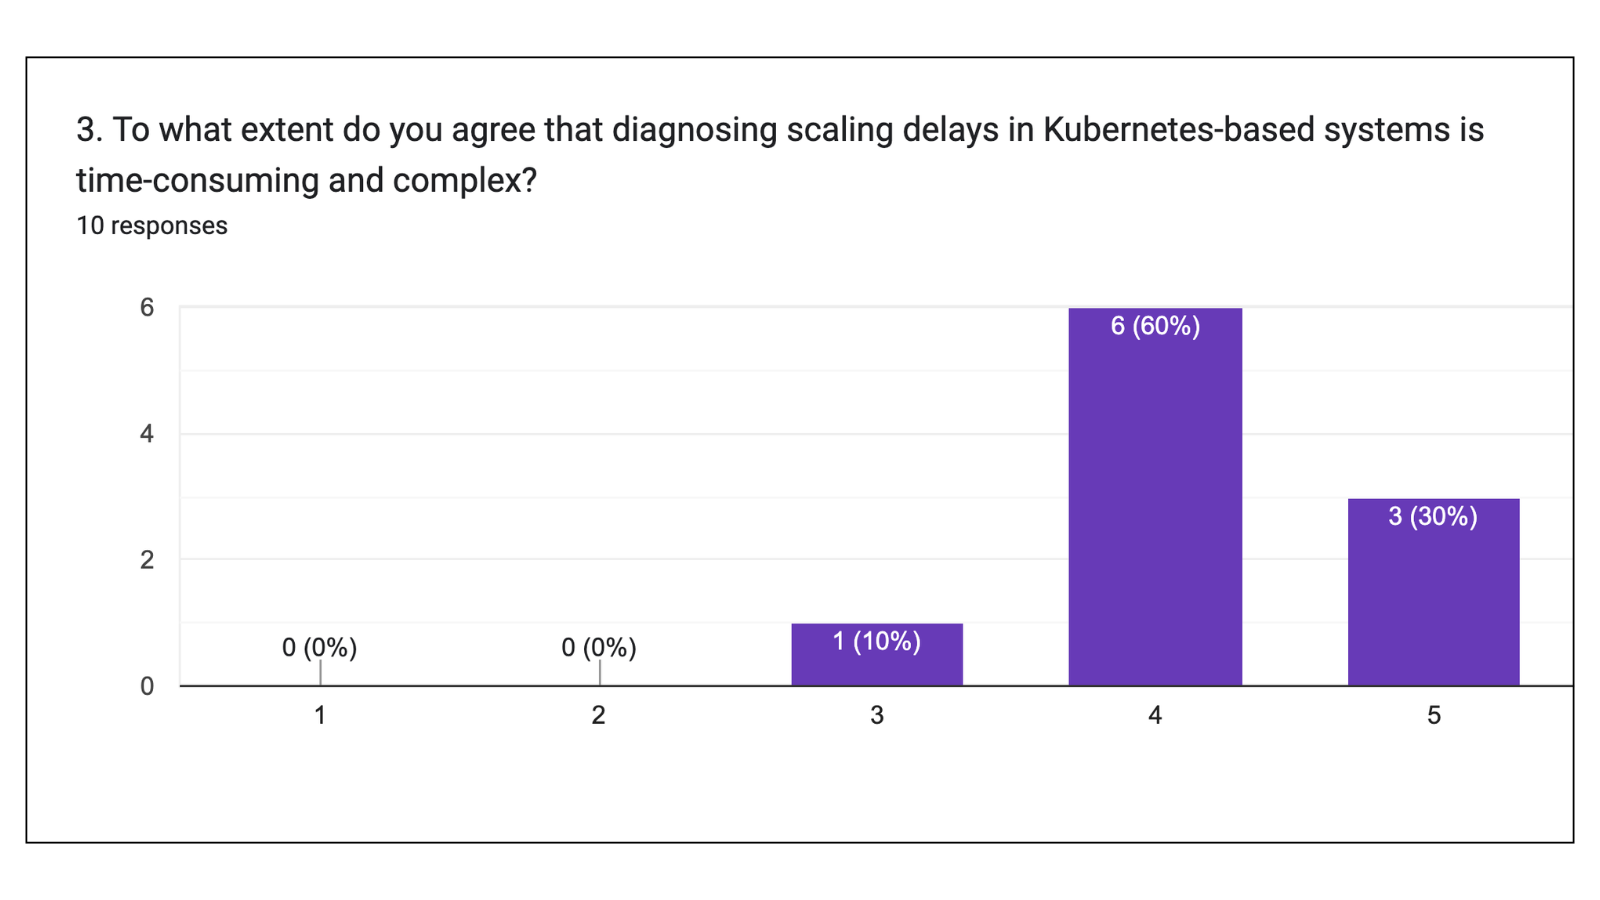
\includegraphics[width=\linewidth]{thesis/assets/question3.png}
&
There is an overwhelming consensus (90\% of respondents giving a 4 or 5) that manual diagnosis is a significant pain point. This high level of agreement establishes a strong need for automated tools like RootLens, as participants acknowledge that the status quo involves high cognitive load and excessive time spent navigating the complexities of Kubernetes scaling.
\\ \hline

\centering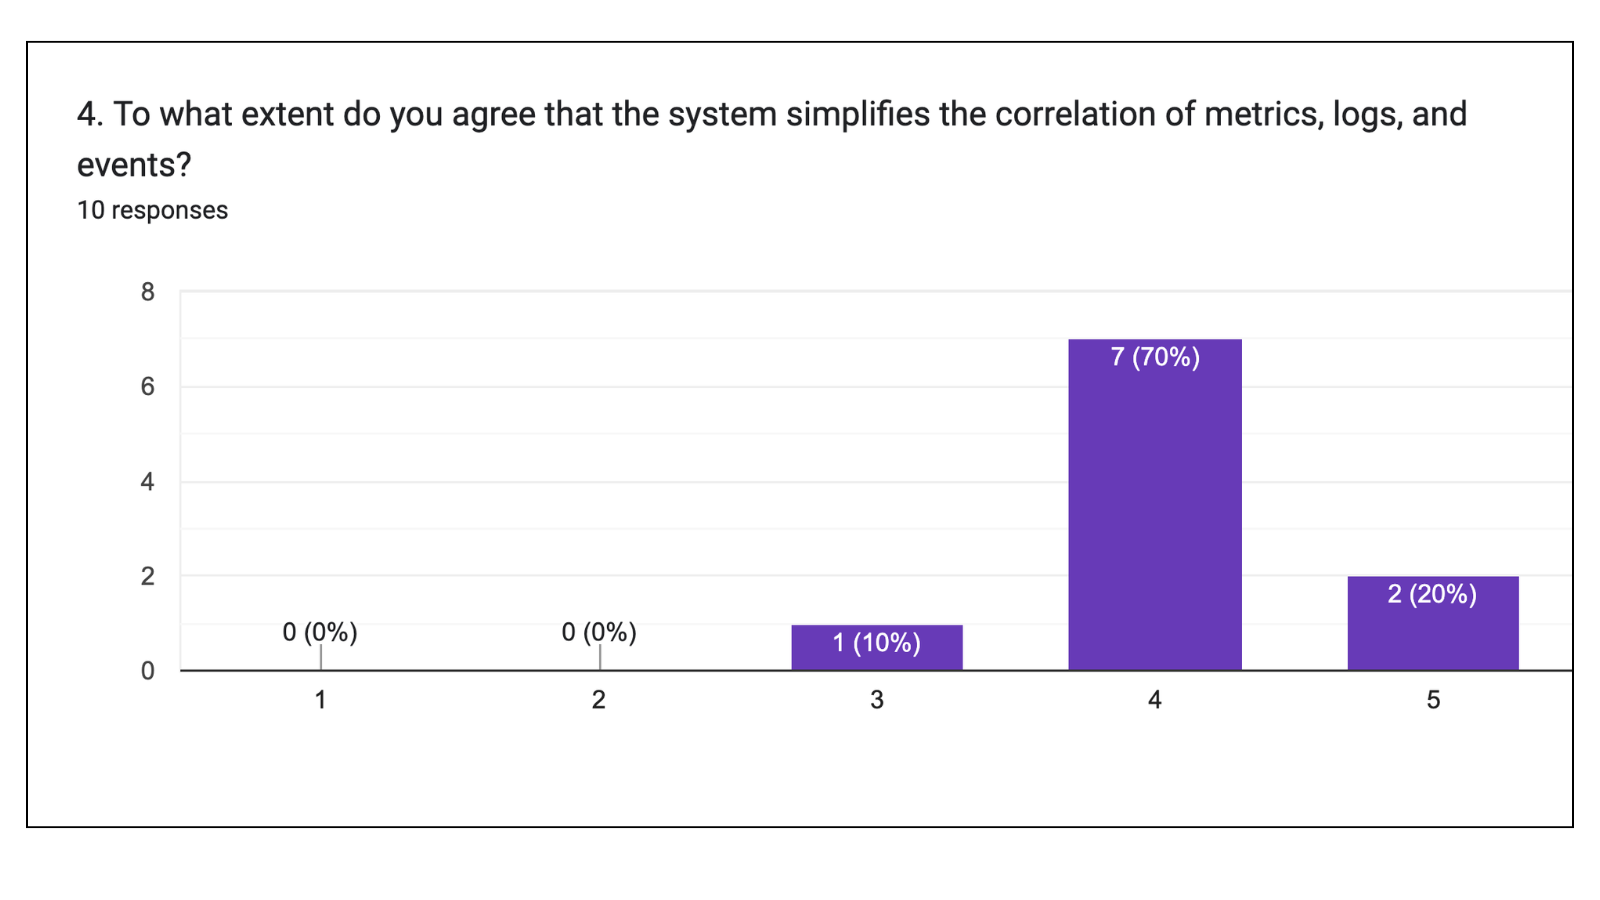
\includegraphics[width=\linewidth]{thesis/assets/question4.png}
&
The system performs exceptionally well in its core technical task, with 90\% of users agreeing that it effectively bridges the gap between different data silos. By successfully correlating metrics, logs, and events, RootLens addresses the primary complexity identified in the previous question, transforming a manual ``needle-in-a-haystack'' search into a streamlined process.
\\ \hline

\centering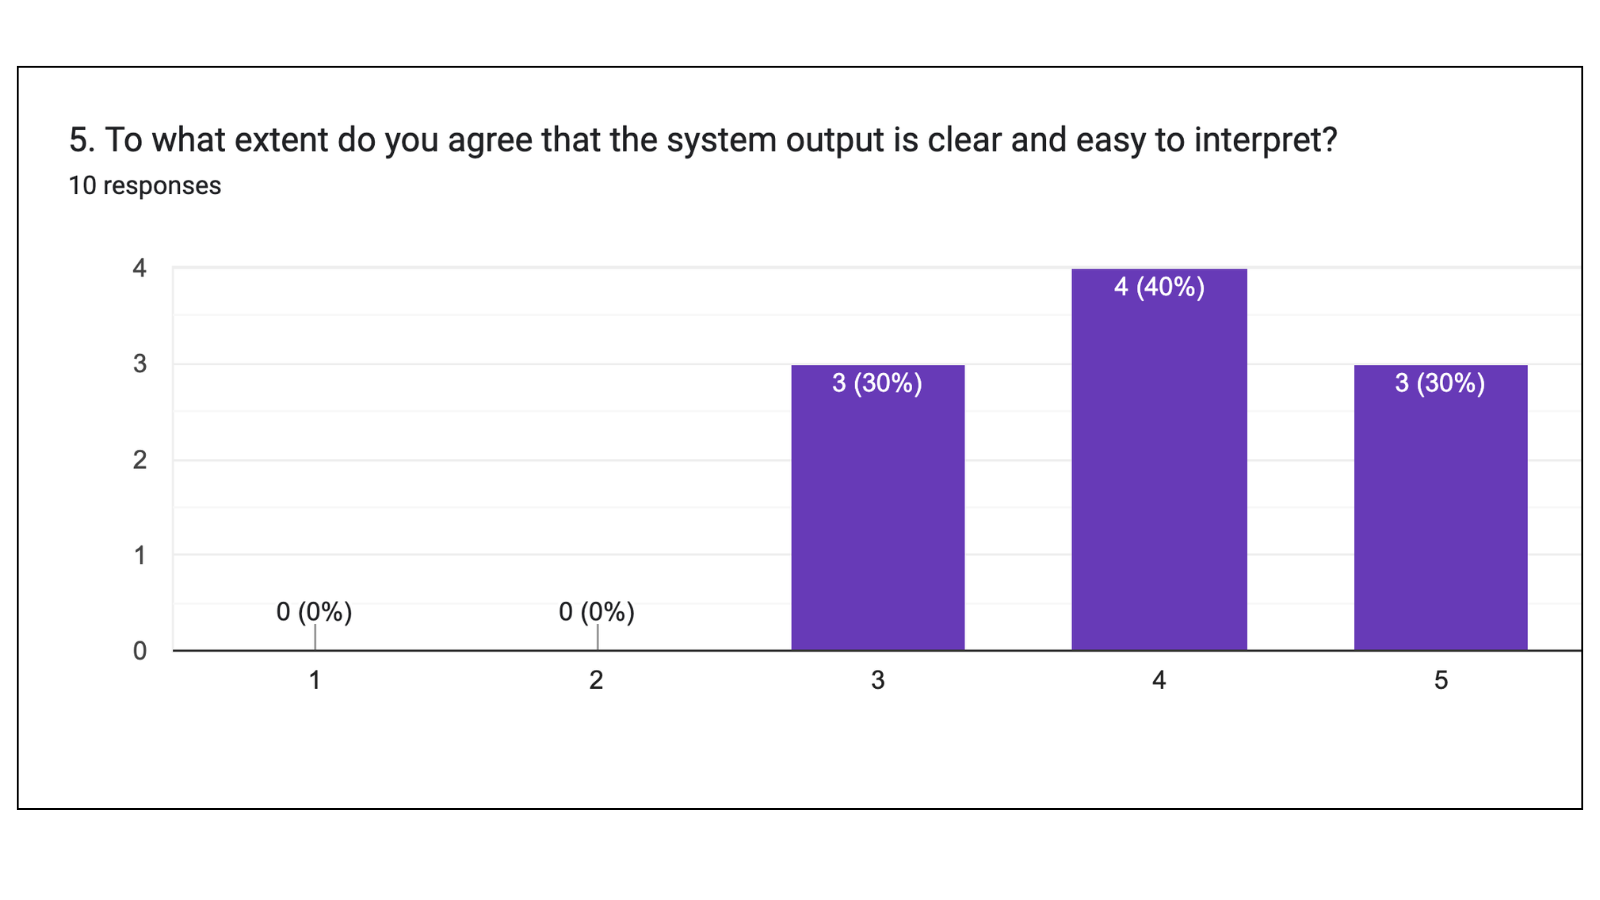
\includegraphics[width=\linewidth]{thesis/assets/question5.png}
&
While the feedback is largely positive (70\% agreement at levels 4 and 5), this area shows the most room for growth compared to the technical correlation. With 30\% of respondents providing a neutral (3) rating, the results suggest that while the system is highly effective at processing data, the presentation layer or the specific wording of the diagnostic explanations could be further refined to ensure total clarity for all user experience levels.
\\ \hline

\end{xltabular}

\begin{table}[H]
\centering
\small
\begin{tabularx}{\textwidth}{|X|c|c|c|c|c|c|}
\hline
\textbf{Evaluation Aspect} & \textbf{Min} & \textbf{Max} & \textbf{Mean} & \textbf{Median} & \textbf{Mode} & \textbf{SD} \\ \hline
Complexity of manual scaling diagnosis (Q3) & 3 & 5 & 4.2 & 4 & 4 & 0.63 \\ \hline
RootLens simplifies event correlation (Q4) & 3 & 5 & 4.1 & 4 & 4 & 0.57 \\ \hline
Clarity of diagnostic outputs (Q5) & 3 & 5 & 4.0 & 4 & 3,4,5 & 0.82 \\ \hline
Overall usefulness of RootLens (Q10) & 4 & 5 & 4.6 & 5 & 5 & 0.52 \\ \hline
\end{tabularx}
\caption{Likert-Scale Evaluation Results ($n=10$)}
\label{tab:likert_results}
\end{table}

All four dimensions achieved mean scores above 4.0, indicating strong agreement. Overall usefulness scored highest (mean 4.6), with all evaluators rating it 4 or 5. Output clarity showed the widest spread (SD=0.82), suggesting varying expectations across experience levels.

\subsection{Qualitative Analysis}
Open-ended responses were coded thematically. Table~\ref{tab:qualitative_feedback} presents representative feedback mapped to evaluation criteria.

\begin{table}[H]
\centering
\small
\begin{tabularx}{\textwidth}{|l|l|X|}
\hline
\textbf{Theme} & \textbf{Evaluator} & \textbf{Representative Feedback} \\ \hline
Visualisation & EV1, EV5 & Dashboard needs timeline visualisation for event correlation and more detailed graphs \\ \hline
Integration & EV3, EV7 & Should integrate with Prometheus, Grafana, and PagerDuty for production workflows \\ \hline
Multi-fault clarity & EV4, EV8 & Output becomes complex when multiple contributing factors are present \\ \hline
Alerting & EV6 & Would benefit from automated alerting for high-confidence diagnoses \\ \hline
Scope & EV2, EV9 & Support for additional KEDA event sources (Kafka, SQS) would increase adoption \\ \hline
Concept validation & EV5, EV7 & Hybrid rule-ML approach is sound; confidence scores are operationally valuable \\ \hline
\end{tabularx}
\caption{Thematic Analysis of Qualitative Feedback}
\label{tab:qualitative_feedback}
\end{table}

\subsection{Domain Expert Feedback}
Domain experts (EV1-EV4, EV6-EV8) confirmed that diagnosing KEDA-triggered scaling delays is a genuine operational challenge, typically requiring 5-30 minutes of manual correlation across Kubernetes events, pod logs, and KEDA metrics. The hybrid rule-ML approach was well-received; experts noted that the sub-cause distinction (e.g., \texttt{slow\_registry} vs.\ \texttt{readiness\_probe\_failure}) maps directly to different remediation actions, which is operationally significant. Confidence scores were identified as particularly valuable for prioritising investigation effort during incidents.

\subsection{Technical Expert Feedback}
Technical experts (EV5, EV9, EV10) assessed the microservice architecture as well-structured, praising the separation of the rule-based engine from the ML service for independent scaling and deployment. The graceful degradation pattern was highlighted as a sound production engineering practice. The JSON-structured diagnostic output was considered production-ready and suitable for integration with monitoring tools. The system scope was judged appropriate for a single-researcher project.

\section{Comparison with Literature}
Toka, Varga and Marosi (2021) achieved over 90\% accuracy using Random Forest for Kubernetes scaling decisions, aligning with RootLens's 96.7\% on a related task. This consistency strengthens the case for Random Forest as a suitable classifier for structured Kubernetes operational data.

Chen et al. (2019) noted struggles with fine-grained failure type distinction, the same challenge RootLens addresses through category-specific models. Decomposing classification into category routing followed by sub-cause prediction avoids the single-model complexity that limits general-purpose outage classification systems.

The chaos engineering approach from Basiri et al. (2016) produced unambiguous ground-truth labels but introduces a validity question: controlled fault injection creates cleaner separations than production, where degradation sources may overlap gradually. The 96.7\% accuracy should be interpreted as an upper bound on expected production performance.

\section{Limitations of Evaluation}
The evaluation has the following limitations:

\begin{enumerate}
    \item \textbf{Small Evaluator Sample:} Ten evaluators provide informed but not statistically generalisable feedback. A larger sample would strengthen the evaluation.
    \item \textbf{Controlled Environment Only:} All experiments were conducted on a single-node Minikube cluster. Production environments with multi-node topologies, different hardware, and concurrent workloads may produce different accuracy profiles.
    \item \textbf{Single Event Source:} The system was validated only with RabbitMQ as the KEDA event source. Other sources (Kafka, AWS SQS) may exhibit different failure patterns requiring threshold recalibration.
    \item \textbf{Small Training Dataset:} 34-42 samples per category limits generalisation confidence. The 100\% held-out test accuracy likely overestimates real-world performance due to the small test sets (6-8 samples).
    \item \textbf{No Long-Duration Testing:} The system was not evaluated under sustained operation over days or weeks, so potential issues such as memory growth in the ring buffer or model drift were not assessed.
\end{enumerate}

\section{Functional and Non-Functional Requirements Implementation}
Table~\ref{tab:fr_status} summarises the implementation status of the functional requirements defined in Chapter~4, and Table~\ref{tab:nfr_status} summarises the non-functional requirements.

\begin{xltabular}{\textwidth}{|p{1.2cm}|p{5cm}|p{2.3cm}|X|}
\hline
\textbf{ID} & \textbf{Requirement} & \textbf{Status} & \textbf{Evidence} \\ \hline
\endfirsthead
\hline
\textbf{ID} & \textbf{Requirement} & \textbf{Status} & \textbf{Evidence} \\ \hline
\endhead
FR01 & Automatically detect KEDA-triggered scaling events & Implemented & Controller watches Kubernetes API for pod creation and ScaledObject state changes \\ \hline
FR02 & Collect timing signals from pod lifecycle events & Implemented & Image pull, scheduling, and readiness probe durations captured \\ \hline
FR03 & Classify scaling delay into three root cause categories & Implemented & Rule-based engine with timing thresholds \\ \hline
FR04 & Extract category-specific feature vector & Implemented & 15/11/10 features extracted per category \\ \hline
FR05 & Invoke category-specific ML explainer model & Implemented & Three Random Forest models via HTTP \\ \hline
FR06 & Compute weighted confidence score ($0.6 \times C_{\text{rule}} + 0.4 \times C_{\text{ml}}$) & Implemented & 60/40 weighted combination \\ \hline
FR07 & Store RCA results in ring buffer (capacity 50) & Implemented & In-memory ring buffer with FIFO eviction \\ \hline
FR08 & REST API endpoint for most recent RCA result & Implemented & JSON API endpoint \\ \hline
FR09 & REST API endpoint for all stored RCA results & Implemented & JSON API endpoint \\ \hline
FR10 & REST API endpoint for aggregate statistics & Implemented & Statistics endpoint with category counts \\ \hline
FR11 & Dashboard displays root cause, sub-cause, confidence, and feature importance & Implemented & React 19 dashboard \\ \hline
FR12 & Dashboard displays historical trend chart & Implemented & Confidence and root cause distribution chart \\ \hline
FR13 & Graceful degradation when ML unavailable & Implemented & Automatic fallback to rule-only mode \\ \hline
FR14 & Health check endpoint for all components & Implemented & Component status endpoint \\ \hline
FR15 & Kubernetes Operator deploys system from single CRD & Implemented & Kubebuilder v4 operator with CRD \\ \hline
\caption{Functional Requirements Implementation Status}
\label{tab:fr_status}
\end{xltabular}

\begin{xltabular}{\textwidth}{|p{1.2cm}|p{3cm}|p{1.8cm}|p{1.8cm}|p{1.5cm}|X|}
\hline
\textbf{ID} & \textbf{Requirement} & \textbf{Target} & \textbf{Achieved} & \textbf{Result} & \textbf{Test Method} \\ \hline
\endfirsthead
\hline
\textbf{ID} & \textbf{Requirement} & \textbf{Target} & \textbf{Achieved} & \textbf{Result} & \textbf{Test Method} \\ \hline
\endhead
NFR01 & RCA latency & $<$ 300ms & 177ms mean & PASS & Timing measurement across 30 experiments \\ \hline
NFR02 & Root cause accuracy & $\geq$ 95\% & 96.7\% & PASS & Fault-injection with ground-truth labels \\ \hline
NFR03 & Sub-cause accuracy & $\geq$ 80\% & 86.7\% & PASS & Fault-injection with ground-truth labels \\ \hline
NFR04 & Concurrent requests & 100 concurrent & Validated & PASS & Load testing with concurrent API calls \\ \hline
NFR05 & HTTPS in production & Required & Implemented & PASS & TLS verification on Cloud Run deployment \\ \hline
NFR06 & No hardcoded credentials & Required & Implemented & PASS & Security audit across 8 config files \\ \hline
NFR07 & K8s 1.28+ portability & Required & Implemented & PASS & Deployment on Minikube with kubebuilder CRD \\ \hline
\caption{Non-Functional Testing Results}
\label{tab:nfr_status}
\end{xltabular}

All functional requirements were implemented and verified through testing. All non-functional requirement targets were met or exceeded.

\section{Chapter Summary}
This chapter critically evaluated RootLens through self-assessment, expert feedback, comparison with existing literature, and requirements traceability. The self-evaluation identified the hybrid architecture and confidence calibration as key strengths, while acknowledging the small dataset and fixed thresholds as limitations. Expert evaluators confirmed the system's industry relevance and practical utility, with suggestions for improved visualisation and broader event source support. All functional and non-functional requirements were satisfied. The identified limitations, particularly the small evaluator sample and controlled-environment-only validation, define the boundaries within which these evaluation results should be interpreted.
